\documentclass[10pt]{beamer}

\usepackage{iftex,ifxetex}
\ifPDFTeX
  \usepackage[utf8]{inputenc}
  \usepackage[T1]{fontenc}
  \usepackage[russian]{babel}
  \usepackage{lmodern}
  \usefonttheme{serif}
\else
  \ifluatex
    \usepackage{unicode-math}
    \defaultfontfeatures{Ligatures=TeX,Numbers=OldStyle}
    \setmathfont{Latin Modern Math}
    \setsansfont{Linux Biolinum O}
    \setmonofont{Fira Code}
    \usefonttheme{professionalfonts}
    % \setmathfont[
    %     Ligatures=TeX,
    %     Scale=MatchLowercase,
    %     math-style=upright,
    %     vargreek-shape=unicode
    %     ]{euler.otf}
  \fi
\fi


\usepackage{amsmath,amssymb,longtable,hhline}
\usepackage{mathrsfs}
\usepackage{xcolor}
\usepackage{listings}
\usepackage{hyperref}
\usepackage{multicol}
\usepackage{anyfontsize}
\usepackage{minted}
%\usepackage{enumitem}

% \setlist[description]{leftmargin=0pt,labelindent=\parindent}

\usemintedstyle{tango}
\newcommand{\ltprgsize}{\fontsize{5}{5}\selectfont}
\setminted{fontsize=\ltprgsize,mathescape}

\definecolor{mygreen}{rgb}{0,0.6,0}
\definecolor{mygray}{rgb}{0.5,0.5,0.5}
\definecolor{mymauve}{rgb}{0.58,0,0.82}

\hypersetup{
    bookmarks=true,         % show bookmarks bar?
    unicode=true,           % non-Latin characters in Acrobat’s bookmarks
    pdftoolbar=false,        % show Acrobat’s toolbar?
    pdfmenubar=false,        % show Acrobat’s menu?
    pdffitwindow=false,     % window fit to page when opened
    pdfstartview={FitH},    % fits the width of the page to the window
    pdftitle={Компьютерная алгебра в задачах оптимизации},    % title
    pdfauthor={Evgeny Cherkashin, Seseg Badmatsyrenova},     % author
    pdfsubject={symbolic computations},   % subject of the document
    pdfnewwindow=true,      % links in new PDF window
    colorlinks=true,       % false: boxed links; true: colored links
    linkcolor=red,          % color of internal links (change box color with linkbordercolor)
    citecolor=green,        % color of links to bibliography
    filecolor=magenta,      % color of file links
    urlcolor=blue           % color of external links
}

\usepackage{pifont}

\usetheme{Warsaw}
\usecolortheme{crane}
%\useinnertheme{rectangles}
\setbeamertemplate{itemize item}{\scriptsize\hbox{\donotcoloroutermaths\ding{113}}}
\setbeamertemplate{itemize subitem}{\tiny\raise1.5pt\hbox{\donotcoloroutermaths$\blacktriangleright$}}
\setbeamertemplate{itemize subsubitem}{\tiny\raise1.5pt\hbox{\donotcoloroutermaths$\blacktriangleright$}}
\setbeamertemplate{enumerate item}{\insertenumlabel.}
\setbeamertemplate{enumerate subitem}{\insertenumlabel.\insertsubenumlabel}
\setbeamertemplate{enumerate subsubitem}{\insertenumlabel.\insertsubenumlabel.\insertsubsubenumlabel}
\setbeamertemplate{enumerate mini template}{\insertenumlabel}

\beamertemplatenavigationsymbolsempty


%\useoutertheme{split}
%\useinnertheme{rounded}
\setbeamertemplate{background canvas}[vertical shading][bottom=white!80!cyan!20,top=cyan!10]
%\setbeamertemplate{sidebar canvas left}[horizontal shading][left=white!40!black,right=black]

\graphicspath{{pics/}}


% --------------------------

% Продукт (Конкуренты, свойства)
% Графический аспект
% Технические аспекты
% Содержание сайта
% Дополнительная информация
% Контактная информация


\begin{document}
\title{Логическое программирование\\ Анализ и понимание текста}

\author{Е.~А.~Черкашин}
\institute[ИДСТУ СО РАН]{ИДСТУ им.~В.~М.~Матросова СО РАН}
\date[2019]{{}\\[1.5cm]
%<<>>\\
26 ноября 2021, Иркутск
}
%\date{\today}
\maketitle


\begin{frame}
  \frametitle{Парадигмы программирования}
  \textbf{Парадигма программирования} (ПП.) -- совокупность идей и понятий, определяющих стиль проектирования компьютерных программ (П.) (подход к программированию);
  способ концептуализации, определяющий организацию вычислений и структурирование работы, выполняемой компьютером (Wikipedia).
  \begin{itemize}
  \item \textbf{Императивная} П. -- последовательность операторов (C, Pascal).
    \begin{itemize}
     \item \textbf{Низкоуровневая} П. -- (1:1) -- управляет непосредственно процессором (Assembler).
     \item \textbf{Конкатенационная} ПП.: операторы (слова) можно ``склеить'' в машинный код (Forth).
     \item \textbf{Структурное} П.: П. и структуры данных представляются \emph{иерархически} (Pascal, C, \ldots).
     \item \textbf{Switch}-П.меняет стратегию поведения при возникновении определенных событий (прием).
    \end{itemize}
  \item \textbf{Функциональная} П. -- суперпозиция функций $prog(x,y) = f(x,g(y,5))$ (LISP, ML, Haskell, OCaML,\ldots).
  \item \textbf{Логическая} П. -- набор высказываний, необходимо доказать истинность (Prolog).
  \end{itemize}
\end{frame}

\begin{frame}
  \frametitle{Парадигмы программирования (продолжение)}
  \begin{itemize}
  \item П. \textbf{Переписывания} -- набор правил замены ``одной строки'' (шаблона) на другую (Рефал).
    \begin{itemize}
      \item \textbf{Макро}-П. -- ``раскрытие'' структур (прием).
      \item \textbf{BDD}\footnote{Binary Decision Diagrams}: ``Раскрытие'' поддеревьев (\TeX, \LaTeX, \ldots).
    \end{itemize}
  \item \textbf{Объектно}-ориентированная П. -- набор объектов, посылающих друг другу сообщения.
    \begin{itemize}
    \item \textbf{Компонентно}-ориентированная -- система состоит из модулей, \emph{интерфейсы} которых доступны во время выполнения \ldots\ (COM+, CORBA, ZCA).
    \item \textbf{Прототипно}-ориентированная: объекты и классы порождаются клонированием (JavaScript, Lua).
    \item \textbf{Агентно}-ориентированная П. -- набор взаимодействующих \emph{агентов}, поведение которых программируется независимо (прием).
    \item \textbf{ Аспектно}-ориентированные инструменты разработки позволяют порождать объекты ООП ``послойно'' (прием, AspectJ).
    \end{itemize}
    \item \textbf{Порождающее} П. -- часть программного кода генерируется из абстрактной модели (прием).
    \item \textbf{Грамотное} П.\footnote{Literate Programming \copyright\ D. Knuth} -- Документация и П. проектируются одновременно (статья в журнале).
  \end{itemize}
\end{frame}

\begin{frame}[fragile]
  \frametitle{Логическое программирование}
  -- ПП., основанная на \emph{автоматическом доказательстве теорем}, а также раздел дискретной математики, изучающий принципы логического вывода \emph{суждений} на основе заданных \emph{фактов} и \emph{правил} вывода.
  \begin{itemize}
  \item ``\verb|%|'' -- комментарий, простирающийся до конца строки,
  \item Программа -- набор фраз (clause):
    \begin{itemize}
    \item факты \\ \verb|works(mario,plumber).|\\\verb|likes(mary,apple).|\\ \verb|contains(sedan,wheel,4).|\\
      \verb|color(apple,red).|\\
      \verb|color(orange,orange).|
    \item правила \\ \verb|likes(kate,X) :-   % ':-' - Если |\\
      \verb|    likes(mary,X), % ',' - И |\\
      \verb|    color(X,red).  % X-переменная|
    \item запросы (суждения) \\ \verb|?- likes(kate, X).|\\\verb|X=apple|.
    \end{itemize}
  \end{itemize}
\end{frame}

\begin{frame}
  \frametitle{QR-код презентации}
  \centering
  \includegraphics[width=0.7\linewidth]{pics/qrcode-log-lang.eps}
\end{frame}

\begin{frame}
  \frametitle{Актуальность понимания естественного языка}
  \footnotesize
  Понимание естественного языка (ЕЯ), перевод из одного ЕЯ на другой -- \textbf{Направление ИИ}. Решаются следующие задачи:
  \begin{enumerate}
  \item Анализ текстов, помещение изъятой информации в базу данных:
    \begin{itemize}
    \item изготовление шаблонов документов, отчетов;
    \item синтез структур данных для ИС;
    \item заполнение баз данных ИС и т.п.;
    \end{itemize}
  \item Ведение диалога с пользователем:
    \begin{itemize}
    \item идентификация моделей и планирование действий (интеллектные пользовательские интерфейсы);
    \item приобретение знаний (оболочки экспертных систем);
    \end{itemize}
  \item Управление приложением:
    \begin{itemize}
    \item запросы на естественном языке к базам данных;
    \item внесение изменений в данные;
    \item командное управление (<<Проветрить квартиру>>).
    \end{itemize}
  \end{enumerate}
  % Цель лекции -- рассмотреть методику использования ЕЯ в качестве языка запросов к базе данных.
\end{frame}

\begin{frame}
  \frametitle{Графический пользовательский интерфейс}
  Специализирован на \textbf{унарных операциях над отдельными частями} информационного объекта.
  \begin{center}
    \includegraphics[width=0.4\linewidth]{pics/shot-context-menu.png}\qquad
    \includegraphics[width=0.4\linewidth]{pics/shot-replace.png}
  \end{center}
  В операциях аргументы вводится в диалоговом окне (для операций с аргументами).

  Более <<умные>> редакторы не используют контекстные операции (EMACS, VI, Visual Studio Code, Sublime, AutoCAD).
\begin{quote}
  \texttt{Alt-X replace-string}, Набирается как <<Alt-X repl str>>
\end{quote}
\begin{center}
    \includegraphics[width=0.9\linewidth]{pics/shot-replace-string-emacs.png}\qquad
  \end{center}
\end{frame}

\begin{frame}
  \frametitle{Язык}
  \begin{block}{Семиотика (наука о знаках) делится на три раздела (Моррис)}
  \begin{itemize}
  \item \textbf{Семантика} — отношение знака к объекту: \\ Что значит \emph{знак}?
  \item \textbf{Синтаксис} — отношение знаков между собой --\\ как создаются \emph{новые смыслы} (термины, суждения) комбинированием \emph{знаков}.
  \item \textbf{Прагматика} — отношение знака к субъекту:\\ Что \emph{обозначает предложение}, что надо дальше делать? На какой конкретно вопрос и как надо отвечать?
  \end{itemize}
\end{block}
\end{frame}

\begin{frame}
  \frametitle{Язык программирования}
\textbf{Синтаксис} на уровне грамматики определяет корректные последовательности символов (операторы, структуры). Но синтаксическая правильность не гарантирует даже осмысленности программы. % Таким образом, синтаксис определяет лишь одну сторону языка.

\textbf{Семантика} — это соответствие между синтаксически правильными программами и [вариантами] действий абстрактного исполнителя, то есть это смысл синтаксических конструкций.

\textbf{Прагматика} задает конкретизацию абстрактного вычислителя (конкретный процессор и др. ресурсы) для  вычислительной системы. Стандарт языка программирования задаёт поведение вычислителя не полностью, конкретный транслятор языка переводит программу в конкретной машинный код на конкретную программно-аппаратную платформу.

Реализованный язык является прагматическим опосредованием абстрактной модели вычислений и ее реализацией на конкретном компьютере.
\vfill
\textbf{Цель программиста} — получить нужный ему эффект в результате исполнения программы на конкретном оборудовании: трансляция и исполнение осуществляется на конкретных вычислителях.

\end{frame}

\begin{frame}
  \frametitle{Синтаксический разбор предложения}
  \begin{center}
    \includegraphics[width=1\linewidth]{pics/morphosent.pdf}
  \end{center}
\end{frame}

\begin{frame}
  \frametitle{Грамматика}
   \begin{columns}
     \begin{column}{0.6\textwidth}
       \begin{block}{}
       \[
         G=\langle T,N,\Sigma,R\rangle
       \]
     \end{block}
       $T$ -- множество терминальных символов (слова, буквы, \texttt{IF}, \texttt{ELSE}),\\
       $N$ -- множество нетерминальных символов (обозначения, $\Alpha, \Beta$, <noun>, <verb>), $T\cap N=\emptyset,$\\
       $\Sigma$ -- стартовый символ (<программа>, <предложение>), $\Sigma\in N,$\\
       $R$ -- множество правил грамматики $\Alpha\to\Beta$, \\$R\subset((T\cup N)^* N(T \cup N)^*)\times(T\cup N)^*$.\\[0.5em]
       Язык $L(G)=\{\Omega\in T^* | \Sigma\to^*\Omega\}$.
     \end{column}
     \begin{column}{0.4\textwidth}
       \begin{block}{Вывод $\Sigma\to^*\Omega$}
         \[\Sigma\to\Sigma\Alpha\quad \Sigma\to\Alpha\]
         \[\Alpha\to b\Sigma e\quad \Alpha\to be \]
         Пример: \(a=`(',\quad b=`)'\).
         \begin{raggedleft}
           \[
             \begin{array}{ll}
               \Sigma & \Sigma\\
               \Alpha & \Alpha\\
               b\Sigma e & ( \Sigma )\\
               b\Sigma\Alpha e & ( \Sigma\Alpha )\\
               b\Alpha\Alpha e & ( \Alpha\Alpha )\\
               bbe\Alpha e & (() \Alpha )\\
               bbebee & (()())
             \end{array} \]
         \end{raggedleft}
     \end{block}
     \end{column}
   \end{columns}
  \begin{center}
    % \includegraphics[width=1\linewidth]{pics/applications-architecture.jpg}
  \end{center}
\end{frame}

\begin{frame}
  \frametitle{Типы грамматик}
  По иерархии Ноама Хомского, грамматики делятся на \textbf{четыре} типа, каждый последующий является более ограниченным подмножеством предыдущего (но и легче поддающимся анализу):
  \begin{itemize}
    \item Тип 0. Неограниченные грамматики — возможны любые правила;
    \item Тип 1. Контекстно-зависимые грамматики — левая часть может содержать один нетерминал, окруженный «контекстом»; сам нетерминал заменяется непустой последовательностью символов в правой части;
    \item Тип 2. Контекстно-свободные грамматики — левая часть состоит из одного нетерминала;
    \item Тип 3. Регулярные грамматики — более простые, распознаются конечными автоматами.
  \end{itemize}
\end{frame}

\begin{frame}[fragile]
  \frametitle{Грамматика языка программирования С}
  {\ltprgsize
 \begin{verbatim}
<translation-unit> ::= {<external-declaration>}*

<external-declaration> ::= <function-definition>
                   | <declaration>

<function-definition> ::= {<declaration-specifier>}* <declarator> {<declaration>}* <compound-statement>
                   | union

<struct-declaration> ::= {<specifier-qualifier>}* <struct-declarator-list>
. . . . . .
<specifier-qualifier> ::= <type-specifier>
                   | <type-qualifier>

<struct-declarator-list> ::= <struct-declarator>
                   | <struct-declarator-list> , <struct-declarator>

<struct-declarator> ::= <declarator>
                   | <declarator> : <constant-expression>
                   | : <constant-expression>
. . . . . .
<selection-statement> ::= if ( <expression> ) <statement>
                   | if ( <expression> ) <statement> else <statement>
                   | switch ( <expression> ) <statement>

<iteration-statement> ::= while ( <expression> ) <statement>
                   | do <statement> while ( <expression> ) ;
                   | for ( {<expression>}? ; {<expression>}? ; {<expression>}? ) <statement>

<jump-statement> ::= goto <identifier> ;
                   | continue ;
                   | break ;
                   | return {<expression>}? ;
\end{verbatim}}
\end{frame}

\begin{frame}[fragile]
  \frametitle{Пример трансляции}
   \begin{columns}
     \begin{column}{0.5\textwidth}
 \begin{minted}{c}
#include <stdio.h>

typedef unsigned long int ulint;

ulint fact (ulint n) {
    if (n==0) return 1;
    if (n==1) return 1;
    return n*fact(n-1);
}

int main() {
    ulint n = 10;
    printf("Factorial of %lu = %lu.\n",
        n, fact(n));
    return 0;
}
 \end{minted}
     \end{column}
      \begin{column}{0.5\textwidth}
\begin{minted}{asm}
	.file   "fact.c"
	.text
	.globl  fact
	.type   fact, @function
fact:
.LFB11:
	movl    $1, %eax
	cmpq    $1, %rdi
	jbe     .L4
.L3:
	imulq   %rdi, %rax
	subq    $1, %rdi
	cmpq    $1, %rdi
	jne    .L3
.L4:
	ret
.LFE11:
	.section    .rodata.str1.1,"aMS",@progbits,1
.LC0:
	.string     "Factorial of %lu = %lu.\n"
	.section    .text.startup,"ax",@progbits
	.globl  main
	.type   main, @function
main:
.LFB12:
	;; . . . . . . . . . . .
	ret
	.cfi_endproc
.LFE12:
	.size   main, .-main
	.ident  "GCC: (GNU) 8.2.1 20181127"
	.section    .note.GNU-stack,"",@progbits
\end{minted}
      \end{column}
    \end{columns}
 \end{frame}

\begin{frame}[fragile]
  \frametitle{Синтаксический разбор предложения}
  Корова трясет хвостом.\\
  A cow shakes the tail.

  \verb|% [a, cow, shakes, the, tail]|

  \textbf{Грамматика:}
  \begin{itemize}
  \item Множество \textbf{терминальных} символов -- \{a,b,c,\ldots,z\}.  На самом деле, $\Sigma=\{a,cow,shakes,walks,\ldots\}$.
  \item Множество \textbf{нетерминальных} символов -- \texttt{<sentence>, <noun>, <verb>, \ldots}
  \item \textnormal{Стартовый} символ -- \texttt{<sentence>}.
  \item \textbf{Правила} упрощенного английского языка:
    \begin{align}
      \label{eq:eng-gramm}
      \langle{}sentence\rangle{} & \to  \langle{}noun group\rangle{} \langle{}verb group\rangle{} \\
      \langle{}noun group\rangle{} & \to  \langle{}determinant\rangle{} \langle{}noun\rangle{} \\
      \langle{}verb group\rangle{} & \to  \langle{}verb\rangle{} \langle{}noun group\rangle{} \\
      \langle{}noun\rangle{} & \to cow\ |\ tail\ |\ \ldots \\
      \langle{}verb\rangle{} & \to walks\ |\ shakes\ |\ \ldots \\
      \langle{}determinant\rangle{} & \to a\ |\ the\ |\ \varepsilon\ |\ my\ |\ \ldots
    \end{align}
  \end{itemize}
\end{frame}

\begin{frame}
  \frametitle{Реализация программы--транслятора}
  \vfil
  \begin{center}
    \Large Пишем программу!
  \end{center}
  \vfil
\end{frame}


% \begin{frame}
%   \frametitle{Графический пользовательский интерфейс}
%   Специализирован на \textbf{унарных операциях над отдельными частями} информационного объекта.
%   \begin{center}
%     \includegraphics[width=0.4\linewidth]{pics/shot-context-menu.png}\qquad
%     \includegraphics[width=0.4\linewidth]{pics/shot-replace.png}
%   \end{center}
%   В операциях аргументы вводится в диалоговом окне (для операций с аргументами).

%   Более <<умные>> редакторы не используют контекстные операции (EMACS, VI, Visual Studio Code, Sublime, AutoCAD).
% \begin{quote}
%   \texttt{Alt-X replace-string}, Набирается как <<Alt-X repl str>>
% \end{quote}
% \begin{center}
%     \includegraphics[width=0.9\linewidth]{pics/shot-replace-string-emacs.png}\qquad
%   \end{center}
% \end{frame}

% \begin{frame}
%   \frametitle{Требования к методике}
%   \textbf{Чего бы мы хотели от такой системы?}
%   \begin{enumerate}
%   \item Представление запросов в терминологии предметной области ИС;
%   \item Выполнение двуаргументных операций над объектами целого класса (не только с экземплярами);
%   \item Система должна синтезировать ответ/действие на основе
%     \begin{itemize}
%     \item введенного запроса/команды на ЕЯ,
%     \item данных и знаний предметной области;
%     \end{itemize}
%   \item Расширяемость/замена предметной области;
%   \item (в идеале) задавать утончающие вопросы;
%   \item (в идеале) обучаться (синонимы, новые декларативные конструкции).
%   \end{enumerate}
% \end{frame}

% \begin{frame}
%   \frametitle{Пакеты прикладных программ}
%   \begin{center}
%     \includegraphics[width=1\linewidth]{pics/applications-architecture.jpg}
%   \end{center}
%   \texttt{input  a.txt multipy by b.txt output c.txt}
% \end{frame}


% \begin{frame}
%   \frametitle{Транслятор языка программирования}
%    \begin{columns}
%      \begin{column}{0.5\textwidth}
%        \includegraphics[width=1\linewidth]{pics/compile-stages.jpg}
%      \end{column}
%      \begin{column}{0.5\textwidth}
%        Внутреннее представление программы -- абстрактное синтаксическое дерево.\\[1em]
%        \includegraphics[width=1\linewidth]{pics/ast-c-main.png}
%      \end{column}
%    \end{columns}
%  \end{frame}


% \begin{frame}[fragile]
%   \frametitle{Трансляция предложений естественного языка}
%    \begin{columns}
%      \begin{column}{0.5\textwidth}
% \begin{minted}{python}
% grammar = nltk.parse_cfg("""
% S  → NP VP
% NP → Det Nom | Det Nom PP | PropN
% Nom → Adj Nom | N
% VP → V | V NP | V NP PP | V S
% PP → P NP

% PropN → 'John' | 'Mary'
% Det → 'the' | 'a'
% N → 'man' | 'woman' | 'park' | 'dog' |
%    'lead' | 'telescope' | 'butterfly'
% Adj  → 'fierce' | 'black' |  'big' |
%    'European'
% V → 'saw' | 'chased' | 'barked'  |
%    'disappeared' | 'said' | 'reported'
% P → 'in' | 'with'
% """)
% \end{minted}
%      \end{column}
%      \begin{column}{0.5\textwidth}
%        \includegraphics[width=0.9\linewidth]{pics/book-tree-14.png}
%        \includegraphics[width=0.9\linewidth]{pics/book-tree-15.png}
%      \end{column}
%    \end{columns}
%  \end{frame}

% \begin{frame}
%   \frametitle{Linked grammar (грамматики связей)}
%   \begin{columns}
%     \begin{column}{0.4\textwidth}
%       \includegraphics[width=0.9\linewidth]{pics/l-g-parts.png}
%       \includegraphics[width=0.9\linewidth]{pics/l-g-table.png}
%     \end{column}
%     \begin{column}{0.6\textwidth}
%       Последовательность слов находится в linked grammar, если существует способ нарисовать связи между словами, такие что\\[1em]
% %      Sequence of words is in the language of link grammar if there is a way to draw links between words in such a way that

%       Связи не пересекаются (\textbf{планарный граф});\\[0.5em]
%       Все слова последовательности соединены связями (\textbf{связность});\\[0.5em]
%       Все связи удовлетворяют ограничениям (\textbf{непротиворечивость})\\[0.5em]
%       Два слова соединены одной и только одной связью (\textbf{исключительность}).\\[0.5em]
%     \end{column}
%   \end{columns}
% \end{frame}

% \begin{frame}
%   \frametitle{Примеры разбора Linked grammar}
%   \centering
%   “The cat chased a snake”\\
%   \includegraphics[width=0.6\linewidth]{pics/l-g-good-ex.png}\\[1em]
%   “The Mary chased cat”\\
%   \includegraphics[width=0.6\linewidth]{pics/l-g-bad-ex.png}
% \end{frame}

% \begin{frame}
%   \frametitle{Примеры разбора Linked grammar}
%   \centering
%   “A dog arrived with a bone”\\
%   “A dog with a bone arrived”\\
%   \includegraphics[width=0.6\linewidth]{pics/l-g-multi-ex.png}\\[1em]
% \end{frame}

% \begin{frame}
%   \frametitle{Примеры разбора Linked grammar}
%   \centering
%   \includegraphics[width=0.8\linewidth]{pics/l-g-prog-ex.png}\\[1em]
% \end{frame}

\begin{frame}[fragile,fragile]
  \frametitle{Информационная система GeoBase. База данных}
  GeoBase -- программа, позволяющая делать запросы на ЕЯ к базе данных по географии США, Borland, 1988.
\begin{minted}{prolog}
state('alabama','al','montgomery',3894e3,51.7e3,22,'birmingham','mobile','montgomery','huntsville').
state('alaska','ak','juneau',401.8e3,591e3,49,'anchorage','fairbanks','juneau','sitka').

city('alabama','al','birmingham',284413).
city('alabama','al','mobile',200452).

border('florida','fl',['georgia','alabama']).

highlow('alabama','al','cheaha mountain',734,'gulf of mexico',0).

mountain('alaska','ak','mckinley',6194).
mountain('alaska','ak','st. elias',5489).

road('66',['district of columbia','virginia']).

lake('huron',59570,['michigan']).
\end{minted}
  {\ttfamily\ltprgsize
\begin{verbatim}


  The database contains the following information:

Information about states:
  Area of the state in square kilometers
  Population of the state in citizens
  Capital of the state
  Which states border a given state
  Rivers in the state
  Cities in the state
  Highest and lowest point in the state in meters

Information about rivers:
  Length of river in kilometers

Information about cities:
  Population of the city in citizens
\end{verbatim}}
\end{frame}

\begin{frame}[fragile]
   \frametitle{Примеры запросов}
{\ttfamily\footnotesize
\begin{verbatim}
Some sample queries:

   - states

   - give me the cities in california.

   - what is the biggest city in california ?

   - what is the longest river in the usa?

   - which rivers are longer than 1 thousand kilometers?

   - what is the name of the state with the lowest point?

   - which states border alabama?

   - which rivers do not run through texas?

   - which rivers run through states that border the state
     with the capital austin?
\end{verbatim}}
\end{frame}

\begin{frame}
  \frametitle{GeoBase}
  \vfil
  \begin{center}
    \Large Смотрим работу GeoBase!
  \end{center}
  \vfil
\end{frame}

\begin{frame}[fragile]
  \frametitle{Схемы (спецификации) интерпретации}
  \begin{columns}
    \begin{column}{0.4\textwidth}
\begin{minted}{prolog}
schema('abbreviation','of','state').
schema('state','with','abbreviation').
schema('capital','of','state').
schema('state','with','capital').
schema('population','of','state').

schema('area','of','state').
schema('city','in','state').

schema('length','of','river').
schema('state','with','river').
schema('river','in','state').

schema('capital','with','population').
schema('point','in','state').

schema('height','of','point').
schema('mountain','in','state').

schema('height','of','mountain').
schema('lake','in','state').

schema('name','of','river').
schema('name','of','capital').

schema('road','in','continent').
\end{minted}
    \end{column}
    \begin{column}{0.6\textwidth}
      \includegraphics[width=1\linewidth]{pics/sem-net-1.pdf}
    \end{column}
  \end{columns}
\end{frame}

\begin{frame}[fragile]
  \frametitle{Программа}
  Основной цикл программы
\begin{minted}{prolog}
geobase(STR, X, E):-
        STR \= "",
        atom_string(ATOM,STR),
        tokenize_atom(ATOM,LIST),     /* Returns a list of words(symbols)           */
        filter(LIST,LIST1),           /* Removes punctuation and words to be ignored*/
        pars(LIST1,E,Q),              /* Parses queries                            */
        findall(A,eval_interp(Q,A),L),
        unik(L,L1),
        % unit(E,U),
        member(X,L1).
\end{minted}
  Синтаксический анализатор (часть)
\begin{minted}{prolog}
  pars(LIST,E,Q):-s_attr(LIST,OL,E,Q),check(OL),!.
  pars(LIST,_,_):-error(LIST),fail.
% . . . . . .
  /* How big is the biggest city -- BIG QUERY */
  s_attr([BIG|S1],S2,E1,q_eaq(E1,A,E2,Q)):-
		size(_,BIG),s_minmax(S1,S2,E2,Q),
		size(E2,BIG),entitysize(E2,E1),
		schema(E1,A,E2),!.

  s_attr(S1,S2,E,Q):-s_minmax(S1,S2,E,Q).
% . . . . . .

/* ... the shortest river in texas -- MIN QUERY */
  s_assoc1([MIN|S1],S2,E1,A,q_eaq(E1,A,E2,q_min(E2,Q))):-minn(MIN),!,
		s_nest(S1,S2,E2,Q),schema(E1,A,E2).

/* ... the longest river in texas -- MAX QUERY */
  s_assoc1([MAX|S1],S2,E1,A,q_eaq(E1,A,E2,q_max(E2,Q))):-maxx(MAX),!,
		s_nest(S1,S2,E2,Q),schema(E1,A,E2).
\end{minted}
\end{frame}

\begin{frame}[fragile]
  \frametitle{Корпус, источник данных}
  \texttt{population of Washington}\\
  Население штата или города?\\
  \textbf{?-} \texttt{schema('population','of','city').}\\
  \textbf{?-} \texttt{schema('population','of','state').}\\
  Корпус реализован при помощи реструктуризации базы данных.
\begin{minted}{prolog}
  % . . . . . . . . .
  /* Relationships about states */
  db(abbreviation,of,state,ABBREVIATION,STATE):-  state(STATE,ABBREVIATION,_,_,_,_,_,_,_,_).
  db(state,with,abbreviation,STATE,ABBREVIATION):-state(STATE,ABBREVIATION,_,_,_,_,_,_,_,_).
  db(area,of,state,AREA,STATE):-        state(STATE,_,_,_,AREA1,_,_,_,_,_),str_real(AREA,AREA1).
  db(capital,of,state,CAPITAL,STATE):-  state(STATE,_,CAPITAL,_,_,_,_,_,_,_).
  db(state,with,capital,STATE,CAPITAL):-state(STATE,_,CAPITAL,_,_,_,_,_,_,_).
  db(population,of,state,POPULATION,STATE):-state(STATE,_,_,POPUL,_,_,_,_,_,_),str_real(POPULATION,POPUL).
  db(state,border,state,STATE1,STATE2):-border(STATE2,_,LIST),member(STATE1,LIST).

  /* Relationships about rivers */
  db(length,of,river,LENGTH,RIVER):-    river(RIVER,LENGTH1,_),str_real(LENGTH,LENGTH1).
  db(state,with,river,STATE,RIVER):-    river(RIVER,_,LIST),member(STATE,LIST).
  db(river,in,state,RIVER,STATE):-      river(RIVER,_,LIST),member(STATE,LIST).

  /* Relationships about points */
  db(point,in,state,POINT,STATE):-      highlow(STATE,_,POINT,_,_,_).
  db(point,in,state,POINT,STATE):-      highlow(STATE,_,_,_,POINT,_).
  db(state,with,point,STATE,POINT):-    highlow(STATE,_,POINT,_,_,_).
  db(state,with,point,STATE,POINT):-    highlow(STATE,_,_,_,POINT,_).
  db(height,of,point,HEIGHT,POINT):-    highlow(_,_,_,_,POINT,H),str_real(HEIGHT,H),!.
  db(height,of,point,HEIGHT,POINT):-    highlow(_,_,POINT,H,_,_),str_real(HEIGHT,H),!.
  % . . . . . . . . .
\end{minted}
\end{frame}

\begin{frame}[fragile]
  \frametitle{Программа}
  Интерпретация запроса \texttt{\ldots findall(A,eval\_interp(Q,A),L), \ldots}
\begin{minted}{prolog}
  eval_interp(Q,IAns):-
		eval(Q,A),
		e_i(A,IAns).

  eval(q_min(ENT,TREE),ANS):-
		findall(X,eval(TREE,X),L),
		entitysize(ENT,ATTR),
		sel_min(ENT,ATTR,99e99,'',ANS,L).

  eval(q_max(ENT,TREE),ANS):-
		findall(X,eval(TREE,X),L),
		entitysize(ENT,ATTR),
		sel_max(ENT,ATTR,-1,'',ANS,L).

  eval(q_sel(E,gt,ATTR,VAL),ANS):-
		schema(ATTR,ASSOC,E),
		db(ATTR,ASSOC,E,SVAL2,ANS),
		str_real(SVAL2,VAL2),
		VAL2>VAL.
% . . . . . . .
  eval(q_eaq(E1,A,E2,TREE),ANS):-
		eval(TREE,VAL),db(E1,A,E2,ANS,VAL).

  eval(q_eaec(E1,A,E2,C),ANS):-db(E1,A,E2,ANS,C).

  eval(q_e(E),ANS):-	ent(E,ANS). % EVAL "ATOM"

  eval(q_or(TREE,_),ANS):- eval(TREE,ANS).

  eval(q_or(_,TREE),ANS):- eval(TREE,ANS).

  eval(q_and(T1,T2),ANS):- eval(T1,ANS1),eval(T2,ANS),ANS=ANS1.
\end{minted}
\end{frame}

% \begin{frame}[fragile]
%   \frametitle{Семантический WEB}
%   В настоящее время появились новые варианты представления предметной области, при этом
%   \begin{itemize}
%   \item сущности идентифицируются, как правило, глобально;
%   \item разработаны стандарты представления информации в конкретных предметных областях (oa, prov, foaf, \ldots);
%   \item стандартизированы базовые онтологии (RDF, RDFs, dc, dcterms), при помощи которых задаются предметные онтологии;
%   \item исследуются свойства логик описаний (DL, SHOIND, \ldots);
%   \item предложены способы;
%   \item созданы форматы представления данных (RDF, RDFa, OWL, JSON-LD, \ldots);
%   \item существуют сервисы предоставления онтологической информации (dbpedia.org, lov.linkeddata.es/dataset/lov/), программное обеспечение создания таких сервисов (ClioPatria);
%   \item язык запросов к онтологическим сервисам (SPARQL), технологии распределенных запросов к сервисам;
%   \item инструментальные средства моделирования предметной области с выдачей в стандартные форматы (Proteg\'e).
%   \end{itemize}
% \end{frame}

% \begin{frame}[fragile]
%   \frametitle{Онтология Open Annotation (oa)}
%   \begin{center}
%     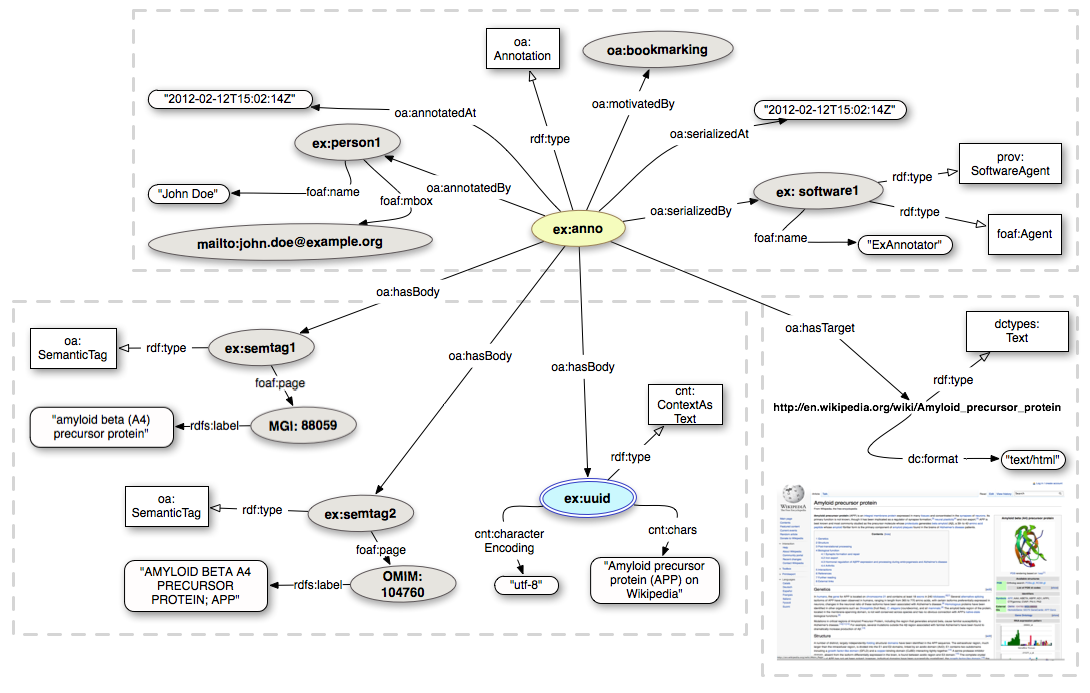
\includegraphics[width=1\linewidth]{pics/Open-Annotation_CB_Bookmarking_and_Semantically_Tagging_A_webpage_spec20130128.png}
%   \end{center}
% \end{frame}

% \begin{frame}[fragile]
%   \frametitle{Инструменты: словарь связных данных (LOV)}
%   \begin{center}
%     \includegraphics[width=0.8\linewidth]{pics/lov-main.png}
%   \end{center}
% \end{frame}

% \begin{frame}[fragile]
%   \frametitle{Инструменты: браузер онтологий}
%   \begin{center}
%     \includegraphics[width=0.8\linewidth]{pics/lov-visual.png}
%   \end{center}
% \end{frame}

% \begin{frame}[fragile]
%   \frametitle{Инструменты: сервер онтологий ClioPatria}
%   \begin{center}
%     \includegraphics[width=0.8\linewidth]{pics/ClioPatria-shot.png}
%   \end{center}
% \end{frame}

% \begin{frame}[fragile]
%   \frametitle{Инструменты: редактор онтологий Proteg\'e}
%   \begin{columns}
%     \begin{column}{0.4\textwidth}
%       \includegraphics[width=1\linewidth]{pics/NLP-fault-tbox-shot.png}
%     \end{column}
%     \begin{column}{0.6\textwidth}
%       \includegraphics[width=1\linewidth]{pics/NLP-fault-abox-shot.png}
%     \end{column}
%   \end{columns}
% \end{frame}

% \begin{frame}[fragile]
%   \frametitle{Модификация GeoBase на основе Semantic WEB}
% \begin{minted}{prolog}
% schema('fault','in','continent').  % Связь с терминами GeoBase
% schema('fault','with','feature').
% schema('name','of','fault').       %
% % schema('feature','of','fault').  % Это отношение находится в T-Box Faults''

% % <<Загрузка>> онтологий
% schema(Prop, 'of', SubjName):-     % используется на этапе трансляции
%         var(SubjName),
%         geob_prop(Prop,_).

% schema(Prop, 'of', SubjName):-     % используется на этапе интерпретации
%         nonvar(SubjName),          % задан конкретный класс
%         geob_prop(Prop, GProp),
%         geob_ent_class(SubjName, Subj),
%         rdf_reachable(Subj, rdfs:subClassOf, Parent),
%         rdf(GProp, rdfs:domain, Parent),!.

% geob_prop(Prop, GProp):-           % Проверка свойства
%         rdf_global_id(geob:Prop, GProp),
%         rdf(GProp,rdf:type,owl:'ObjectProperty'),!.

% geob_class(Class, GClass):-        % Проверка класса
%         rdf_global_id(geob:Class, GClass),
%         rdf(GClass,rdf:type,owl:'Class'),!.

% geob_ent_class(Ent, Class):-
%         sub_atom(Ent,0,1,R,H),
%         sub_atom(Ent,1,R,0,T),
%         string_upper(H,U),
%         atom_concat(U,T,GEnt),
%         geob_class(GEnt, Class).

% geob_ent(E, A):-
%         nonvar(E),
%         geob_ent_class(E,Class),
%         rdf(A, rdf:type, Class, geodata). % Сущность онтологии geodata
% \end{minted}
% \end{frame}

% \begin{frame}[fragile]
%   \frametitle{Интерфейс пользователя GeoBase + ActiveFaults}
%   \begin{center}
%     \includegraphics[width=1\linewidth]{pics/Geobase-ui.png}
%   \end{center}
% \end{frame}

% \begin{frame}[fragile]
%   \frametitle{Схемы данных из моделей ИС}
%   В разработке программного обеспечения используются модели, представляющие объекты, бизнес-процессы и организационную систему предприятия (UML-2.4, SysML, BPMN-2.0, CMMN).
%   \begin{enumerate}
%   \item Формирование модели при помощи редакторов;
%   \item Экспорт модели в формат XMI;
%   \item Преобразование XMI в формат онтологии \verb|<subject, predicate, object>|;
%   \item Преобразование базы данных в формат онтологии, или реализация адаптера;
%   \item Настройка связей с основной схемой данных;
%   \item Настройка корпуса, который также можно организовать при помощи адаптера базы данных.
%   \end{enumerate}
% \end{frame}

\begin{frame}
  \frametitle{Заключение}
  Чтобы компьютер понимал, что хочет пользователь надо реализовать следующие модели:
  \begin{enumerate}
  \item Грамматику языка (синтаксис),
  \item Семантику его элементов,
  \item Прагматику:
    \begin{itemize}
    \item Соответствие предложений языка смыслам и действиям, для этого всегда требуется,
    \item Модель предметной области.
    \end{itemize}
  \end{enumerate}
  \begin{columns}
    \begin{column}{0.5\linewidth}
      Актуальные (хайповые) проекты по теме -- программирование \textbf{навыков} голосовых помощников (Алиса, Маруся, Сири, G-Ноу, Алекса, Робин, Сяо-Ай, Олег, Дуся, Горыныч, Тайп, Агрегат).\\[1em]
      Умный дом.
    \end{column}
    \begin{column}{0.6\linewidth}
      \includegraphics[width=\linewidth]{pics/flat.jpg}
    \end{column}
  \end{columns}
\end{frame}

\begin{frame}
  \vfill
  \begin{center}
    {\Huge Спасибо за внимание!}
  \end{center}
  \vfill
%  Исходный код (без документации) доступен на github.com: \url{https://github.com/isu-enterprise/icc.xmitransform}, \url{https://github.com/eugeneai/icc.mothurpim}.
\end{frame}
\begin{frame}
  \frametitle{QR-код презентации}
  \centering
  \includegraphics[width=0.7\linewidth]{pics/qrcode-log-lang.eps}
\end{frame}

\end{document}

%%% Local Variables:
%%% mode: latex
%%% TeX-master: t
%%% End:
